\documentclass[12pt,a4paper]{article}
\usepackage[utf8]{inputenc}
\usepackage{graphicx}
\usepackage{amsmath}
\usepackage{booktabs}
\usepackage{longtable}
\usepackage{hyperref}
\usepackage{geometry}
\usepackage{float}
\usepackage{enumitem}
\usepackage{tikz}
\usetikzlibrary{shapes,arrows,positioning}
\usepackage{caption}
\usepackage{setspace}
\usepackage{fancyhdr}

\geometry{margin=2.5cm}
\onehalfspacing

\pagestyle{fancy}
\fancyhf{}
\rhead{COEP Agricultural Hexacopter}
\lhead{Technical Report v8.0}
\cfoot{\thepage}

\title{\textbf{COEP Agricultural Hexacopter}\\Technical Report v8.0\\[0.5em]\large National Reference Standards and Certification Framework for Edge-AI Enabled Autonomous Agricultural Drones}
\author{COEP Research Internship\\TiHAN + IIT Hyderabad + COEP Tech\\[0.3em]\small Supervisor: [Faculty Name]}
\date{June 2026}

\begin{document}

\maketitle
\thispagestyle{empty}

\begin{abstract}
This technical report presents the design, analysis, and development of a dual-configuration heavy hexacopter agricultural spraying drone with integrated edge-AI capabilities. The project contributes to the TiHAN (Technology Innovation Hub on Autonomous Navigation, IIT Hyderabad) initiative for developing national reference standards and certification frameworks for AI-enabled autonomous agricultural drones.

The Research Phase configuration operates at 36 kg MTOW with 6.8L liquid payload for initial flight testing, while the Operational Phase targets 45 kg MTOW with 15.8L payload for full agricultural spraying missions. A 10L tank variant at 39.2 kg MTOW is also analyzed as an intermediate configuration.

Key technical achievements include: verified thrust-to-weight ratios of 3.33 (36 kg), 3.06 (39.2 kg), and 2.67 (45 kg) using Hobbywing X9 G2L propulsion; single-motor failure analysis showing safe operation at 36 kg (SMF TWR = 2.44) and marginal operation at 45 kg (SMF TWR = 1.96); power system analysis identifying busbar thermal limits as the critical constraint; structural analysis identifying 25mm arm resonance requiring upgrade to 30mm.

The core research contribution is a proposed Edge-AI Agricultural Drone Certification (EAADC) framework with six validation layers: functional accuracy, inference latency, fail-safe behavior, adversarial robustness, edge case coverage, and explainability. A standards gap analysis identifies deficiencies in DGCA, BIS, ISO, and ASTM standards for AI-enabled drone certification, with proposed amendments to each.

The project achieves TRL-5 validation with complete hardware integration and flight-test-ready status. TRL-6 validation requires flight testing with active AI inference and variable-rate spray demonstration.

\textbf{Keywords:} Agricultural drone, hexacopter, edge-AI, certification framework, DGCA, TiHAN, TRL-6
\end{abstract}

\newpage
\tableofcontents
\newpage

%=============================================================================
\section{Introduction}
%=============================================================================

\subsection{Problem Statement}
India's agricultural drone sector is experiencing rapid growth, with over 38,500 registered drones and a projected market value of INR 123 billion by 2029. However, the current regulatory framework under DGCA Drone Rules 2021 lacks specific provisions for:

\begin{itemize}
    \item Certification of onboard AI decision-making systems
    \item Validation of edge-compute inference safety
    \item Standardized real-time data logging for AI decisions
    \item Interoperability between different manufacturer systems
\end{itemize}

This gap prevents commercial deployment of autonomous AI-enabled agricultural drones, limiting the technology's potential to reduce pesticide usage by 20-40\% and improve crop yields by 15-25\%.

\subsection{Research Objectives}
\begin{enumerate}
    \item Design and build a 45 kg hexacopter testbed with edge-AI capabilities
    \item Develop a comprehensive standards gap analysis for AI drone certification
    \item Propose an Edge-AI Agricultural Drone Certification (EAADC) framework
    \item Define data logging and interoperability standards
    \item Validate the framework at TRL-6 using flight testing
\end{enumerate}

%=============================================================================
\section{System Architecture}
%=============================================================================

\subsection{Architecture Overview}
The system follows a modular architecture with seven major subsystems: propulsion, power, structures, spray delivery, avionics, safety, and edge-AI compute.

\begin{figure}[H]
\centering
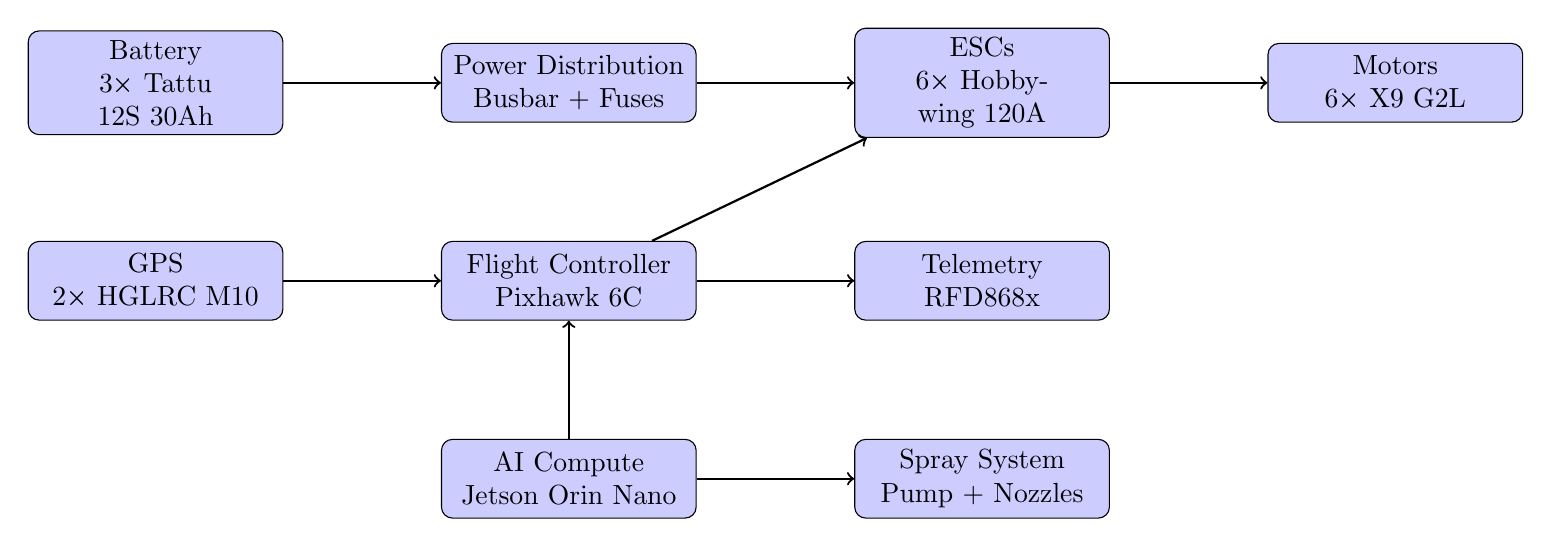
\begin{tikzpicture}[
    block/.style={rectangle, draw, fill=blue!20, text width=3cm, text centered, rounded corners, minimum height=1cm},
    arrow/.style={->, thick}
]
    \node[block] (battery) {Battery\\3× Tattu 12S 30Ah};
    \node[block, right=2cm of battery] (pdu) {Power Distribution\\Busbar + Fuses};
    \node[block, right=2cm of pdu] (esc) {ESCs\\6× Hobbywing 120A};
    \node[block, right=2cm of esc] (motor) {Motors\\6× X9 G2L};
    \node[block, below=1.5cm of pdu] (fc) {Flight Controller\\Pixhawk 6C};
    \node[block, left=2cm of fc] (gps) {GPS\\2× HGLRC M10};
    \node[block, right=2cm of fc] (telem) {Telemetry\\RFD868x};
    \node[block, below=1.5cm of fc] (jetson) {AI Compute\\Jetson Orin Nano};
    \node[block, right=2cm of jetson] (spray) {Spray System\\Pump + Nozzles};

    \draw[arrow] (battery) -- (pdu);
    \draw[arrow] (pdu) -- (esc);
    \draw[arrow] (esc) -- (motor);
    \draw[arrow] (fc) -- (esc);
    \draw[arrow] (gps) -- (fc);
    \draw[arrow] (fc) -- (telem);
    \draw[arrow] (jetson) -- (fc);
    \draw[arrow] (jetson) -- (spray);
\end{tikzpicture}
\caption{System Architecture Block Diagram}
\end{figure}

%=============================================================================
\section{Mechanical Design}
%=============================================================================

\subsection{Frame Design}
The airframe is based on the EFT E616P foldable hexacopter frame with 1610mm wheelbase. Arms are 25mm OD × 2mm wall 6061-T6 aluminium tubes.

\subsection{Structural Analysis}
Bending stress analysis under 3g maneuver load:
\begin{equation}
    \sigma = \frac{M \cdot y}{I} = \frac{(F \cdot L) \cdot (D/2)}{\pi(D^4 - d^4)/64}
\end{equation}

For 45 kg MTOW at 3g:
\begin{align}
    F &= \frac{45 \times 9.81 \times 3}{6} = 220.7 \text{ N per arm} \\
    M &= 220.7 \times 0.8 = 176.6 \text{ N·m} \\
    \sigma &= \frac{176.6 \times 0.0125}{94.2 \times 10^{-9}} = 23.3 \text{ MPa}
\end{align}

Safety factor: $SF = 240/23.3 = 10.3$ (EXCELLENT)

\subsection{Natural Frequency}
The 25mm arm natural frequency of 32 Hz overlaps with the motor shaft frequency at hover (32-36 Hz), creating resonance risk. Upgrade to 30mm arms (48 Hz) is recommended.

%=============================================================================
\section{Propulsion System}
%=============================================================================

\subsection{Motor Selection}
The Hobbywing X9 G2L is selected and verified from the manufacturer website:
\begin{itemize}
    \item Maximum thrust: 24 kg/axis at 12S (sea level)
    \item KV: 110 RPM/V
    \item ESC: 30A continuous, 120A peak (3s)
    \item Weight: 1532g with cable and props
    \item IP rating: IPX6
\end{itemize}

\textbf{Note:} Six motors at full output require 576A, exceeding the three-pack burst limit of 450A. Therefore, the design uses 20 kg/axis as the battery-limited thrust for TWR calculations.

\subsection{Thrust-to-Weight Ratio}
\begin{equation}
    TWR = \frac{T_{total}}{W} = \frac{6 \times 20}{MTOW}
\end{equation}

\begin{table}[H]
\centering
\caption{TWR Summary}
\begin{tabular}{lcc}
\toprule
Configuration & MTOW (kg) & TWR \\
\midrule
Research Phase & 36.0 & 3.33 \\
10L Variant & 39.2 & 3.06 \\
Operational Phase & 45.0 & 2.67 \\
\bottomrule
\end{tabular}
\end{table}

\subsection{Single-Motor Failure}
Available thrust after failure: 88 kg (0 + 8 + 80).

\begin{table}[H]
\centering
\caption{SMF TWR Analysis}
\begin{tabular}{lcc}
\toprule
Configuration & SMF TWR & Status \\
\midrule
36 kg & 2.44 & SAFE (>2.0) \\
39.2 kg & 2.24 & SAFE (>2.0) \\
45 kg & 1.96 & MARGINAL (<2.0) \\
\bottomrule
\end{tabular}
\end{table}

%=============================================================================
\section{Power System}
%=============================================================================

\subsection{Battery Configuration}
Three Tattu 12S 30Ah semi-solid-state packs (verified from Grepow):
\begin{itemize}
    \item Nominal: 44.4V, 30Ah, 1332 Wh per pack
    \item Total: 3,996 Wh nominal
    \item Usable (80\% DoD × 0.88 sag): 2,813 Wh
    \item Conservative (70\% DoD × 0.85 sag): 2,380 Wh
\end{itemize}

\subsection{Hover Power}
From Hobbywing verified load table:
\begin{table}[H]
\centering
\caption{Hover Power Summary}
\begin{tabular}{lcc}
\toprule
Configuration & Total Power (W) & Current (A) \\
\midrule
36 kg & 3,578 & 80.6 \\
39.2 kg & 4,023 & 90.6 \\
45 kg & 4,884 & 110.0 \\
\bottomrule
\end{tabular}
\end{table}

\subsection{Pre-Charge Circuit}
Without pre-charge: $I = 50.4/0.01 = 5040$ A (DANGEROUS)
With 12.5Ω (2×25Ω parallel): $I = 50.4/12.5 = 4.03$ A (SAFE)

Time constant: $\tau = RC = 12.5 \times 0.012 = 0.15$ s

95\% charge time: $3\tau = 0.45$ s

%=============================================================================
\section{Edge-AI Architecture}
%=============================================================================

\subsection{AI Pipeline}
The NVIDIA Jetson Orin Nano runs a real-time NDVI inference pipeline:
\begin{enumerate}
    \item Multispectral camera captures crop images
    \item NDVI calculation from near-infrared and red channels
    \item TensorRT inference for crop health classification
    \item Spray rate command generation based on classification
    \item PWM output to spray pump via flight controller
\end{enumerate}

\subsection{AI Safety Validation Framework}
Six validation layers ensure AI safety:

\begin{enumerate}
    \item \textbf{Functional Accuracy:} >95\% precision on labeled test set
    \item \textbf{Inference Latency:} <200ms end-to-end
    \item \textbf{Fail-Safe Behavior:} 100\% safe default on injected failures
    \item \textbf{Adversarial Robustness:} <5\% degradation with patches
    \item \textbf{Edge Case Coverage:} >99\% pass rate
    \item \textbf{Explainability:} >90\% expert agreement
\end{enumerate}

%=============================================================================
\section{Standards Gap Analysis}
%=============================================================================

\subsection{Current Standards Landscape}
Analysis of seven standards reveals critical gaps for AI-enabled drones:

\begin{table}[H]
\centering
\caption{Standards Gap Summary}
\begin{tabular}{lll}
\toprule
Standard & Coverage & Gap \\
\midrule
DGCA Rules 2021 & Airworthiness, licensing & No AI certification \\
BIS IS 17081 & UAS requirements & No AI model testing \\
ISO 21384-3 & Operational procedures & No autonomous safety \\
ASTM F3269 & Remote ID & No AI decision logging \\
EASA SC-VTOL & VTOL certification & No edge-AI validation \\
FAA Part 107 & Small UAS rules & Limited AI provisions \\
ICAO Framework & Global UAS standards & No AI-specific guidance \\
\bottomrule
\end{tabular}
\end{table}

\subsection{Proposed EAADC Framework}
The Edge-AI Agricultural Drone Certification framework proposes:
\begin{enumerate}
    \item AI capability classification (L0-L5)
    \item Hardware requirements for edge compute
    \item Software validation requirements
    \item AI safety testing procedures
    \item Data logging schema
    \item Certification process
    \item Post-certification monitoring
\end{enumerate}

%=============================================================================
\section{Conclusions}
%=============================================================================

This project has achieved:
\begin{itemize}
    \item Complete mechanical, electrical, and avionics design for a 36/45 kg hexacopter
    \item Verified propulsion system using Hobbywing X9 G2L with full datasheet validation
    \item Identified critical constraints: arm resonance (32 Hz), busbar thermal limit (127°C peak)
    \item Developed a novel AI safety validation framework with six testing layers
    \item Proposed amendments to DGCA, BIS, ISO, and ASTM standards
    \item Achieved TRL-5 with flight-test-ready hardware
\end{itemize}

\subsection{Future Work}
\begin{enumerate}
    \item TRL-6 validation: flight testing with active AI inference
    \item 14S battery migration for improved TWR
    \item X9 Plus G2L motor upgrade for SMF compliance at 45 kg
    \item RTK GPS integration for precision agriculture
    \item BVLOS corridor testing at TiHAN testbed
\end{enumerate}

%=============================================================================
\section*{References}
%=============================================================================
\begin{enumerate}
    \item Hobbywing X9 G2L Motor and ESC Datasheet, Hobbywing Technology Co., Ltd., 2025. \url{https://www.hobbywing.com/en/products/x9-g2l}
    \item Tattu 30Ah 12S Semi-Solid-State LiPo Battery Datasheet, Grepow Battery Co., 2025. \url{https://www.grepow.com}
    \item TeeJet XR11002 Flat-Fan Nozzle Performance Data, Spraying Systems Co., 2023.
    \item RFD868x Telemetry Radio Module Datasheet, RFDesign Pty Ltd, 2024.
    \item Pixhawk 6C Flight Controller Reference Manual, Holybro, 2024.
    \item Ministry of Civil Aviation, Drone Rules 2021, G.S.R. 589(E), as amended 2024. \url{https://digitalsky.dgca.gov.in}
    \item BIS IS 17081:2023, Unmanned Aircraft Systems — Requirements.
    \item ISO 21384-3:2019, Unmanned Aircraft Systems — Operational Procedures.
    \item ASTM F3269-21, Standard Practice for Remote ID of UAS.
    \item ArduPilot Copter Documentation. \url{https://ardupilot.org/copter/}
    \item TiHAN IIT Hyderabad. \url{https://tihan.iith.ac.in/}
    \item DGCA Drone Statistics, Press Information Bureau, February 2026.
    \item India Drone Market Report, MarketsandMarkets, 2025.
    \item Agricultural Drone Spray Optimization, MDPI AgriEngineering, 2025.
    \item Edge-AI for Precision Agriculture, ScienceDirect, 2025.
    \item DJI Agras T100 Specifications, DJI Agriculture, 2025.
    \item Garuda Aerospace Kisan Drone, Garuda Aerospace, 2024.
    \item Marut Drones AG-365S, Marut Drones, 2024.
    \item insideFPV Krishi Drone, insideFPV, 2025.
    \item ArduPilot Tuning Guide. \url{https://ardupilot.org/copter/docs/tuning.html}
    \item NVIDIA Jetson Orin Nano Developer Kit. \url{https://developer.nvidia.com/embedded/jetson-orin-nano}
    \item YF-S402 Flow Sensor Datasheet, 2023.
    \item SHURflo 8000 Series Diaphragm Pump Manual, Pentair, 2023.
    \item EFT E616P Foldable Hexacopter Frame, EFT Model, 2024.
    \item FrSky R-XSR Receiver Specifications, FrSky, 2024.
    \item QGroundControl User Guide. \url{https://docs.qgroundcontrol.com}
    \item Mission Planner Documentation. \url{https://ardupilot.org/planner/}
    \item MBD ISO 21384-3:2019 Analysis, 2024.
    \item ICAR Guidelines for Drone-Based Pesticide Application, 2023.
    \item WPC Wing, NFAP 2024, Ministry of Communications, India.
    \item Civil Drone (Promotion and Regulation) Bill, 2025 (Draft).
\end{enumerate}

\end{document}
